% Options for packages loaded elsewhere
\PassOptionsToPackage{unicode}{hyperref}
\PassOptionsToPackage{hyphens}{url}
%
\documentclass[
]{article}
\usepackage{lmodern}
\usepackage{amssymb,amsmath}
\usepackage{ifxetex,ifluatex}
\ifnum 0\ifxetex 1\fi\ifluatex 1\fi=0 % if pdftex
  \usepackage[T1]{fontenc}
  \usepackage[utf8]{inputenc}
  \usepackage{textcomp} % provide euro and other symbols
\else % if luatex or xetex
  \usepackage{unicode-math}
  \defaultfontfeatures{Scale=MatchLowercase}
  \defaultfontfeatures[\rmfamily]{Ligatures=TeX,Scale=1}
\fi
% Use upquote if available, for straight quotes in verbatim environments
\IfFileExists{upquote.sty}{\usepackage{upquote}}{}
\IfFileExists{microtype.sty}{% use microtype if available
  \usepackage[]{microtype}
  \UseMicrotypeSet[protrusion]{basicmath} % disable protrusion for tt fonts
}{}
\makeatletter
\@ifundefined{KOMAClassName}{% if non-KOMA class
  \IfFileExists{parskip.sty}{%
    \usepackage{parskip}
  }{% else
    \setlength{\parindent}{0pt}
    \setlength{\parskip}{6pt plus 2pt minus 1pt}}
}{% if KOMA class
  \KOMAoptions{parskip=half}}
\makeatother
\usepackage{xcolor}
\IfFileExists{xurl.sty}{\usepackage{xurl}}{} % add URL line breaks if available
\IfFileExists{bookmark.sty}{\usepackage{bookmark}}{\usepackage{hyperref}}
\hypersetup{
  pdftitle={An Introduction to Modelling Soccer Matches in R (part 2)},
  pdfauthor={Robert Hickman},
  hidelinks,
  pdfcreator={LaTeX via pandoc}}
\urlstyle{same} % disable monospaced font for URLs
\usepackage[margin=1in]{geometry}
\usepackage{color}
\usepackage{fancyvrb}
\newcommand{\VerbBar}{|}
\newcommand{\VERB}{\Verb[commandchars=\\\{\}]}
\DefineVerbatimEnvironment{Highlighting}{Verbatim}{commandchars=\\\{\}}
% Add ',fontsize=\small' for more characters per line
\usepackage{framed}
\definecolor{shadecolor}{RGB}{248,248,248}
\newenvironment{Shaded}{\begin{snugshade}}{\end{snugshade}}
\newcommand{\AlertTok}[1]{\textcolor[rgb]{0.94,0.16,0.16}{#1}}
\newcommand{\AnnotationTok}[1]{\textcolor[rgb]{0.56,0.35,0.01}{\textbf{\textit{#1}}}}
\newcommand{\AttributeTok}[1]{\textcolor[rgb]{0.77,0.63,0.00}{#1}}
\newcommand{\BaseNTok}[1]{\textcolor[rgb]{0.00,0.00,0.81}{#1}}
\newcommand{\BuiltInTok}[1]{#1}
\newcommand{\CharTok}[1]{\textcolor[rgb]{0.31,0.60,0.02}{#1}}
\newcommand{\CommentTok}[1]{\textcolor[rgb]{0.56,0.35,0.01}{\textit{#1}}}
\newcommand{\CommentVarTok}[1]{\textcolor[rgb]{0.56,0.35,0.01}{\textbf{\textit{#1}}}}
\newcommand{\ConstantTok}[1]{\textcolor[rgb]{0.00,0.00,0.00}{#1}}
\newcommand{\ControlFlowTok}[1]{\textcolor[rgb]{0.13,0.29,0.53}{\textbf{#1}}}
\newcommand{\DataTypeTok}[1]{\textcolor[rgb]{0.13,0.29,0.53}{#1}}
\newcommand{\DecValTok}[1]{\textcolor[rgb]{0.00,0.00,0.81}{#1}}
\newcommand{\DocumentationTok}[1]{\textcolor[rgb]{0.56,0.35,0.01}{\textbf{\textit{#1}}}}
\newcommand{\ErrorTok}[1]{\textcolor[rgb]{0.64,0.00,0.00}{\textbf{#1}}}
\newcommand{\ExtensionTok}[1]{#1}
\newcommand{\FloatTok}[1]{\textcolor[rgb]{0.00,0.00,0.81}{#1}}
\newcommand{\FunctionTok}[1]{\textcolor[rgb]{0.00,0.00,0.00}{#1}}
\newcommand{\ImportTok}[1]{#1}
\newcommand{\InformationTok}[1]{\textcolor[rgb]{0.56,0.35,0.01}{\textbf{\textit{#1}}}}
\newcommand{\KeywordTok}[1]{\textcolor[rgb]{0.13,0.29,0.53}{\textbf{#1}}}
\newcommand{\NormalTok}[1]{#1}
\newcommand{\OperatorTok}[1]{\textcolor[rgb]{0.81,0.36,0.00}{\textbf{#1}}}
\newcommand{\OtherTok}[1]{\textcolor[rgb]{0.56,0.35,0.01}{#1}}
\newcommand{\PreprocessorTok}[1]{\textcolor[rgb]{0.56,0.35,0.01}{\textit{#1}}}
\newcommand{\RegionMarkerTok}[1]{#1}
\newcommand{\SpecialCharTok}[1]{\textcolor[rgb]{0.00,0.00,0.00}{#1}}
\newcommand{\SpecialStringTok}[1]{\textcolor[rgb]{0.31,0.60,0.02}{#1}}
\newcommand{\StringTok}[1]{\textcolor[rgb]{0.31,0.60,0.02}{#1}}
\newcommand{\VariableTok}[1]{\textcolor[rgb]{0.00,0.00,0.00}{#1}}
\newcommand{\VerbatimStringTok}[1]{\textcolor[rgb]{0.31,0.60,0.02}{#1}}
\newcommand{\WarningTok}[1]{\textcolor[rgb]{0.56,0.35,0.01}{\textbf{\textit{#1}}}}
\usepackage{graphicx,grffile}
\makeatletter
\def\maxwidth{\ifdim\Gin@nat@width>\linewidth\linewidth\else\Gin@nat@width\fi}
\def\maxheight{\ifdim\Gin@nat@height>\textheight\textheight\else\Gin@nat@height\fi}
\makeatother
% Scale images if necessary, so that they will not overflow the page
% margins by default, and it is still possible to overwrite the defaults
% using explicit options in \includegraphics[width, height, ...]{}
\setkeys{Gin}{width=\maxwidth,height=\maxheight,keepaspectratio}
% Set default figure placement to htbp
\makeatletter
\def\fps@figure{htbp}
\makeatother
\setlength{\emergencystretch}{3em} % prevent overfull lines
\providecommand{\tightlist}{%
  \setlength{\itemsep}{0pt}\setlength{\parskip}{0pt}}
\setcounter{secnumdepth}{-\maxdimen} % remove section numbering

\title{An Introduction to Modelling Soccer Matches in R (part 2)}
\author{Robert Hickman}
\date{2019-06-05}

\begin{document}
\maketitle

In \href{https://www.robert-hickman.eu/post/dixon_coles_1/}{part 1}
we've seen how we can use the Poisson distribution to estimate the
relative strengths of teams in a hypothetical summer league between
Arsenal, Blackburn Rovers, Coventry City, Dover Athletic, Enfield Town,
and Frimley Green. Now we want to move onto actually \emph{using} these
estimates to predict matches, and eventually, whole leagues.

A good way to sum up this post in one line is a quote (mis) attributed
to Niels Bohr:

\hypertarget{its-difficult-to-make-predictions-especially-about-the-future}{%
\subsubsection{\texorpdfstring{\emph{``It's Difficult to Make
Predictions, Especially About the
Future''}}{``It's Difficult to Make Predictions, Especially About the Future''}}\label{its-difficult-to-make-predictions-especially-about-the-future}}

We've made our predictions about the past (estimating the relative
strengths of teams based on past results), now we need to predict the
future. I think it also nicely captures that even our predictions about
the past are noisy- we can not ever truly know the exact strengths of
football teams; the job of analytics is to estimate these are accurately
as possible. But any noise in those past predictions will be carried
forward and amplified when predicting the future.

Onward to the code, first as always, loading libraries and setting a
seed for reproducibility:

\begin{Shaded}
\begin{Highlighting}[]
\KeywordTok{library}\NormalTok{(tidyverse)}

\KeywordTok{set.seed}\NormalTok{(}\DecValTok{3459}\NormalTok{)}
\end{Highlighting}
\end{Shaded}

We're then going to load all the stuff we prepped and predicted in the
last post. Remember the α parameter below referse to a teams attacking
strength (the relative number of goals they are expected to score), and
the β parameter referse to the attacking strength (the inverse of the
relative number of goals they are expected to concede). Finally, γ
referse to the extra advantage of playing at home.

\begin{Shaded}
\begin{Highlighting}[]
\NormalTok{fixtures <-}\StringTok{ }\KeywordTok{readRDS}\NormalTok{(}\StringTok{"../../static/files/dc_fixtures.rds"}\NormalTok{)}
\NormalTok{results <-}\StringTok{ }\KeywordTok{readRDS}\NormalTok{(}\StringTok{"../../static/files/dc_results.rds"}\NormalTok{)}

\NormalTok{model <-}\StringTok{ }\KeywordTok{readRDS}\NormalTok{(}\StringTok{"../../static/files/dc_model.rds"}\NormalTok{)}

\NormalTok{model}
\end{Highlighting}
\end{Shaded}

\begin{verbatim}
## $alpha
##          Arsenal Blackburn_Rovers    Coventry_City   Dover_Athletic 
##        1.1106558        0.6370160        0.3023048       -0.2875353 
##     Enfield_Town    Frimley_Green 
##       -0.3767038       -1.3857376 
## 
## $beta
##          Arsenal Blackburn_Rovers    Coventry_City   Dover_Athletic 
##        0.6457175        0.4289270        0.3647815       -0.1362931 
##     Enfield_Town    Frimley_Green 
##       -0.3852812       -0.9178517 
## 
## $gamma
##    gamma 
## 0.189462
\end{verbatim}

We'll define a quick function to do our prediction. For a quick
explanation of exactly why it's coded as presented, see
\href{https://www.robert-hickman.eu/post/dixon_coles_1/\#Tinkering}{the
previous post}, under the title `Tinkering'.

For a given string of a home team and an away team, the function finds
the relevant parameters from a third argument (param\_list) and
calculates the expected goal for each team.

\begin{Shaded}
\begin{Highlighting}[]
\NormalTok{predict_results <-}\StringTok{ }\ControlFlowTok{function}\NormalTok{(home, away, param_list) \{}
\NormalTok{  e_goals_home <-}\StringTok{ }\KeywordTok{exp}\NormalTok{(param_list}\OperatorTok{$}\NormalTok{alpha[home] }\OperatorTok{-}\StringTok{ }\NormalTok{param_list}\OperatorTok{$}\NormalTok{beta[away] }\OperatorTok{+}\StringTok{ }\NormalTok{param_list}\OperatorTok{$}\NormalTok{gamma)}
\NormalTok{  e_goals_away <-}\StringTok{ }\KeywordTok{exp}\NormalTok{(param_list}\OperatorTok{$}\NormalTok{alpha[away] }\OperatorTok{-}\StringTok{ }\NormalTok{param_list}\OperatorTok{$}\NormalTok{beta[home])}
  
\NormalTok{  df <-}\StringTok{ }\KeywordTok{data.frame}\NormalTok{(}\DataTypeTok{home =}\NormalTok{ home, }\DataTypeTok{away =}\NormalTok{ away,}
                   \DataTypeTok{e_hgoal =} \KeywordTok{as.numeric}\NormalTok{(e_goals_home), }
                   \DataTypeTok{e_agoal =} \KeywordTok{as.numeric}\NormalTok{(e_goals_away))}
  
  \KeywordTok{return}\NormalTok{(df)}
\NormalTok{\}}
\end{Highlighting}
\end{Shaded}

If we run this for two example teams for example:

\begin{Shaded}
\begin{Highlighting}[]
\CommentTok{#two example teams}
\NormalTok{home <-}\StringTok{ "Blackburn_Rovers"}
\NormalTok{away <-}\StringTok{ "Arsenal"}

\NormalTok{prediction <-}\StringTok{ }\KeywordTok{predict_results}\NormalTok{(home, away, model) }
\NormalTok{prediction}
\end{Highlighting}
\end{Shaded}

\begin{verbatim}
##               home    away  e_hgoal  e_agoal
## 1 Blackburn_Rovers Arsenal 1.198128 1.977293
\end{verbatim}

We can see that it gives Arsenal (the away team) a slightly more
optimistic chance than Blackburn. The expected goals for each team of
course can be rewritten as the mean, and in our Poisson model refers to
λ (lambda)- the mean times an event (goal) happens per a time interval
(match). We also set a maximum number of possible goals (7 in this
case*) to bound the area under the distribution so we aren't sampling
forever.

*sharp readers might notice that this is actually \emph{lower} than the
lambda for our more extreme cases (e.g.~Arsenal at home to Frimley
Green), but for realistic matches (even between wildly different
professional sides) this is a fair enough assumption.

We then use dpois() to calculate the probability of this Poisson
function returning a value (0:7 goals) given it's lambda value. So if we
run this over the prediction we made for Blackburn Rovers vs.~Arsenal we
get:

\begin{Shaded}
\begin{Highlighting}[]
\CommentTok{#set a limit of where we'll calculate across}
\NormalTok{max_goals <-}\StringTok{ }\DecValTok{7}

\CommentTok{#calculate the probability of scoring x goals for either team}
\NormalTok{blackburn_goal_probs <-}\StringTok{ }\KeywordTok{lapply}\NormalTok{(}\DecValTok{0}\OperatorTok{:}\NormalTok{max_goals, dpois, }\DataTypeTok{lambda =}\NormalTok{ prediction}\OperatorTok{$}\NormalTok{e_hgoal)}
\NormalTok{arsenal_goal_probs <-}\StringTok{ }\KeywordTok{lapply}\NormalTok{(}\DecValTok{0}\OperatorTok{:}\NormalTok{max_goals, dpois, }\DataTypeTok{lambda =}\NormalTok{ prediction}\OperatorTok{$}\NormalTok{e_agoal)}

\CommentTok{#bind together in a df}
\NormalTok{df <-}\StringTok{ }\KeywordTok{data.frame}\NormalTok{(}\DataTypeTok{goals =} \KeywordTok{rep}\NormalTok{(}\DecValTok{0}\OperatorTok{:}\NormalTok{max_goals, }\DecValTok{2}\NormalTok{),}
                 \DataTypeTok{team =} \KeywordTok{rep}\NormalTok{(}\KeywordTok{c}\NormalTok{(home, away), }\DataTypeTok{each =}\NormalTok{ max_goals}\OperatorTok{+}\DecValTok{1}\NormalTok{),}
                 \DataTypeTok{p =} \KeywordTok{c}\NormalTok{(}\KeywordTok{unlist}\NormalTok{(blackburn_goal_probs), }\KeywordTok{unlist}\NormalTok{(arsenal_goal_probs)))}

\CommentTok{#plot the p of scoring x goals for either team}
\NormalTok{p1 <-}\StringTok{ }\KeywordTok{ggplot}\NormalTok{(df, }\KeywordTok{aes}\NormalTok{(}\DataTypeTok{x =}\NormalTok{ goals, }\DataTypeTok{y =}\NormalTok{ p, }\DataTypeTok{fill =}\NormalTok{ team)) }\OperatorTok{+}
\StringTok{  }\KeywordTok{geom_density}\NormalTok{(}\DataTypeTok{stat =} \StringTok{"identity"}\NormalTok{, }\DataTypeTok{alpha =} \FloatTok{0.5}\NormalTok{) }\OperatorTok{+}
\StringTok{  }\KeywordTok{scale_fill_manual}\NormalTok{(}\DataTypeTok{values =} \KeywordTok{c}\NormalTok{(}\StringTok{"red"}\NormalTok{, }\StringTok{"blue"}\NormalTok{)) }\OperatorTok{+}
\StringTok{  }\KeywordTok{labs}\NormalTok{(}\DataTypeTok{title =} \StringTok{"Predicted goals for Blackburn Rovers and Arsenal"}\NormalTok{,}
       \DataTypeTok{y =} \StringTok{"probability"}\NormalTok{) }\OperatorTok{+}
\StringTok{  }\KeywordTok{theme_minimal}\NormalTok{()}

\NormalTok{p1}
\end{Highlighting}
\end{Shaded}

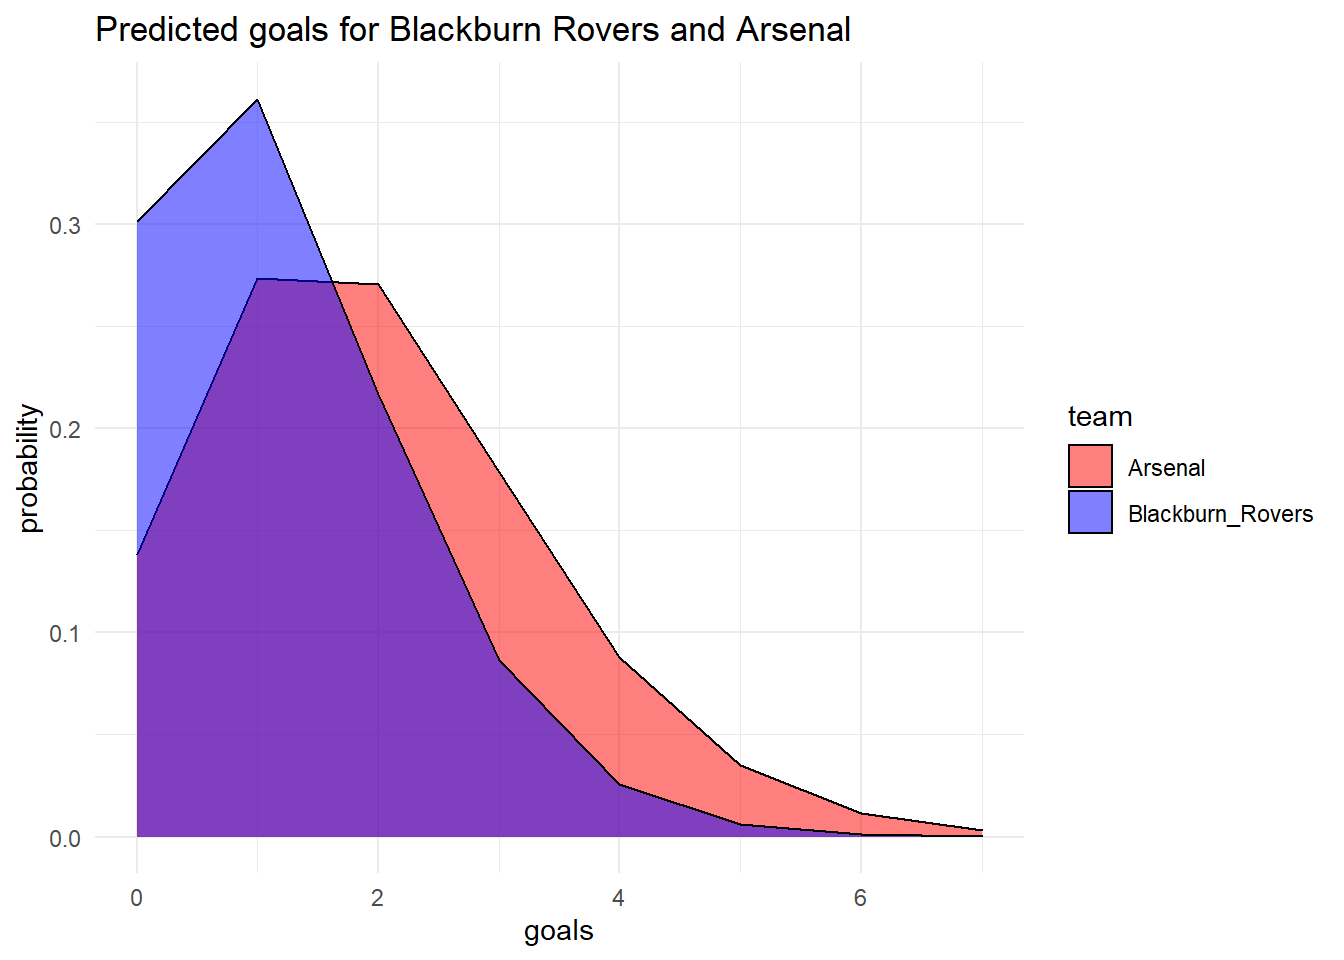
\includegraphics{2019-30-5-dixon-coles-2_files/figure-latex/predict_mach_goals-1.pdf}

Because of how maths works, these curves are the same result we would
get if we ran rpois() (sampling from the Poisson function) lots of
times. We'll do that quickly because it sets the stage nicely for what
will come later.

\begin{Shaded}
\begin{Highlighting}[]
\CommentTok{#sample from the function lots of times for each team}
\NormalTok{n <-}\StringTok{ }\DecValTok{100000}
\NormalTok{blackburn_goals_samples <-}\StringTok{ }\KeywordTok{rpois}\NormalTok{(n, }\DataTypeTok{lambda =}\NormalTok{ prediction}\OperatorTok{$}\NormalTok{e_hgoal)}
\NormalTok{arsenal_goals_samples <-}\StringTok{ }\KeywordTok{rpois}\NormalTok{(n, }\DataTypeTok{lambda =}\NormalTok{ prediction}\OperatorTok{$}\NormalTok{e_agoal)}

\NormalTok{df <-}\StringTok{ }\KeywordTok{data.frame}\NormalTok{(}\DataTypeTok{team =} \KeywordTok{rep}\NormalTok{(}\KeywordTok{c}\NormalTok{(home, away), }\DataTypeTok{each =}\NormalTok{ n),}
                 \DataTypeTok{sampled_goals =} \KeywordTok{c}\NormalTok{(blackburn_goals_samples, arsenal_goals_samples))}

\CommentTok{#look its the same plot!}
\NormalTok{p2 <-}\StringTok{ }\KeywordTok{ggplot}\NormalTok{(df, }\KeywordTok{aes}\NormalTok{(}\DataTypeTok{x =}\NormalTok{ sampled_goals, }\DataTypeTok{fill =}\NormalTok{ team)) }\OperatorTok{+}
\StringTok{  }\KeywordTok{geom_bar}\NormalTok{(}\DataTypeTok{stat =} \StringTok{"count"}\NormalTok{, }\DataTypeTok{position =} \StringTok{"dodge"}\NormalTok{, }\DataTypeTok{colour =} \StringTok{"black"}\NormalTok{, }\DataTypeTok{alpha =} \FloatTok{0.5}\NormalTok{) }\OperatorTok{+}
\StringTok{  }\KeywordTok{geom_line}\NormalTok{(}\KeywordTok{aes}\NormalTok{(}\DataTypeTok{colour =}\NormalTok{ team), }\DataTypeTok{stat =} \StringTok{"count"}\NormalTok{, }\DataTypeTok{size =} \DecValTok{3}\NormalTok{) }\OperatorTok{+}
\StringTok{  }\KeywordTok{scale_fill_manual}\NormalTok{(}\DataTypeTok{values =} \KeywordTok{c}\NormalTok{(}\StringTok{"red"}\NormalTok{, }\StringTok{"blue"}\NormalTok{), }\DataTypeTok{guide =} \OtherTok{FALSE}\NormalTok{) }\OperatorTok{+}
\StringTok{  }\KeywordTok{scale_colour_manual}\NormalTok{(}\DataTypeTok{values =} \KeywordTok{c}\NormalTok{(}\StringTok{"red"}\NormalTok{, }\StringTok{"blue"}\NormalTok{), }\DataTypeTok{guide =} \OtherTok{FALSE}\NormalTok{) }\OperatorTok{+}
\StringTok{  }\KeywordTok{labs}\NormalTok{(}\DataTypeTok{title =} \StringTok{"Predicted goals for Blackburn Rovers and Arsenal"}\NormalTok{,}
       \DataTypeTok{y =} \StringTok{"probability"}\NormalTok{,}
       \DataTypeTok{x =} \StringTok{"sampled goals"}\NormalTok{) }\OperatorTok{+}
\StringTok{  }\KeywordTok{theme_minimal}\NormalTok{() }\OperatorTok{+}
\StringTok{  }\KeywordTok{theme}\NormalTok{(}\DataTypeTok{axis.text.y =} \KeywordTok{element_blank}\NormalTok{())}

\NormalTok{p2}
\end{Highlighting}
\end{Shaded}

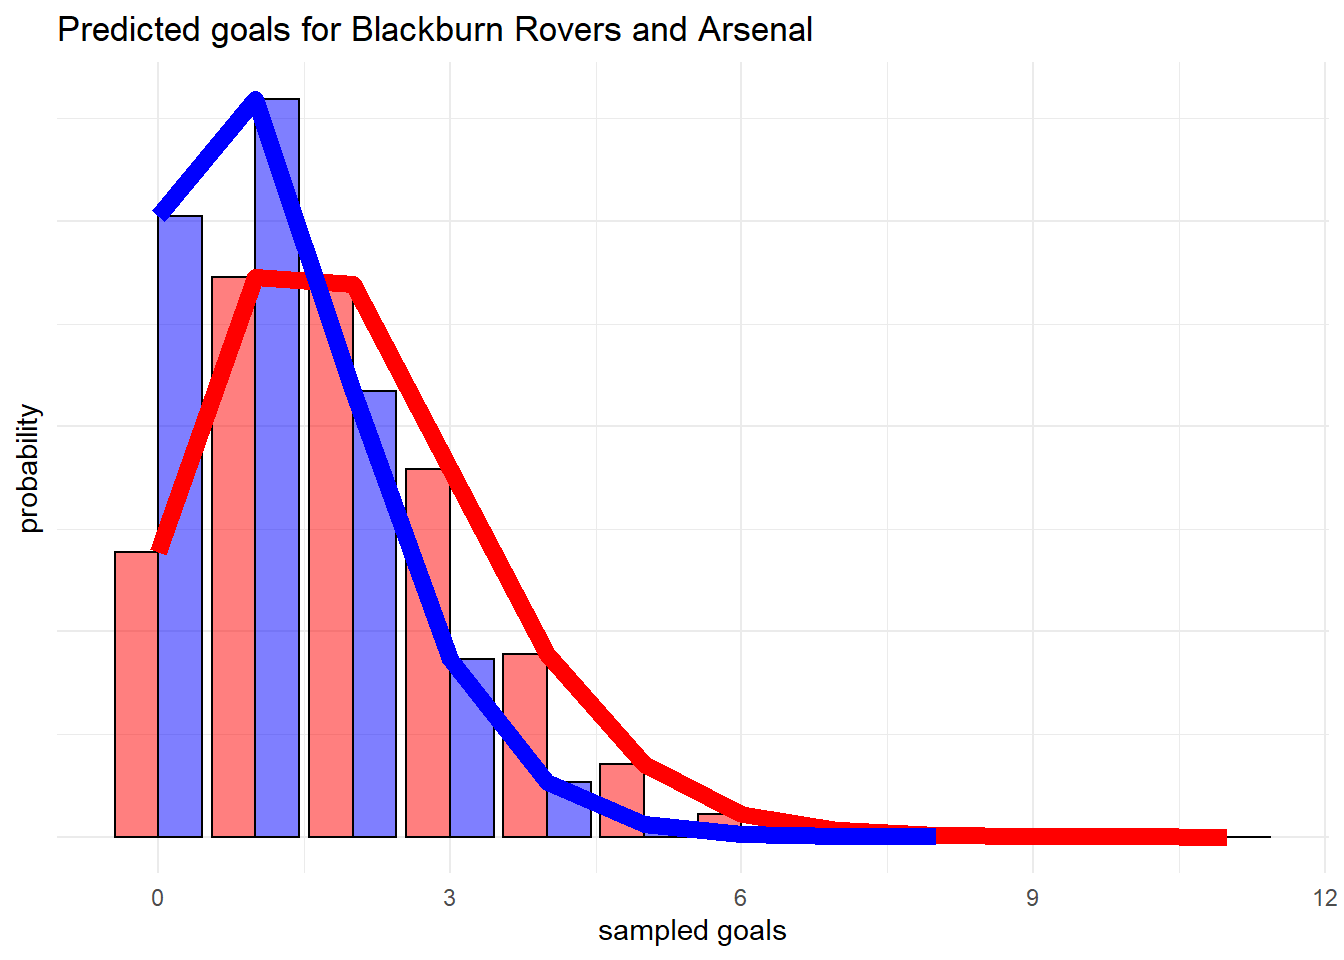
\includegraphics{2019-30-5-dixon-coles-2_files/figure-latex/monte_carlo_poisson-1.pdf}

Ok great!, in terms of predicting the result, the rightwards shift of
the red (Arsenal) curve here is the difference in the teams ability to
generate a positive goal differential- it makes it more likely that if
we sample event, Arsenal will have scored more goals than Blackburn
Rovers at the end of the match. Of course, it's also obvious that while
Arsenal's curve is right shifted, the bars for Arsenal scoring 0 goals
and Blackburn scoring 6 are still sizeable enough that it isn't outside
the realm of possibility.

This is a nice way ofpresenting the chance of each team scoring n goals,
but doesn't really help us in predicting the result of a match given
that this relies on the interaction of both these distributions (we need
to know how many goals BOTH Arsenal AND Blackburn will score).

To calculate this, we can do an outer product of the probabilities for
both teams scoring n goals. We can then plot the probability of each
\emph{scoreline} as a tile plot:

\begin{Shaded}
\begin{Highlighting}[]
\CommentTok{#calculate matrix of possible results and probabilities of those}
\NormalTok{matrix <-}\StringTok{ }\KeywordTok{outer}\NormalTok{(}\KeywordTok{unlist}\NormalTok{(arsenal_goal_probs), }\KeywordTok{unlist}\NormalTok{(blackburn_goal_probs)) }\OperatorTok
\StringTok{  }\KeywordTok{as.data.frame}\NormalTok{() }\OperatorTok
\StringTok{  }\KeywordTok{gather}\NormalTok{() }\OperatorTok
\StringTok{  }\CommentTok{#add in scorelines}
\StringTok{  }\KeywordTok{mutate}\NormalTok{(}\DataTypeTok{hgoals =} \KeywordTok{rep}\NormalTok{(}\DecValTok{0}\OperatorTok{:}\NormalTok{max_goals, max_goals}\OperatorTok{+}\DecValTok{1}\NormalTok{),}
         \DataTypeTok{agoals =} \KeywordTok{rep}\NormalTok{(}\DecValTok{0}\OperatorTok{:}\NormalTok{max_goals, }\DataTypeTok{each =}\NormalTok{ max_goals}\OperatorTok{+}\DecValTok{1}\NormalTok{))}

\CommentTok{#make the tile plot}
\NormalTok{p3 <-}\StringTok{ }\KeywordTok{ggplot}\NormalTok{(matrix, }\KeywordTok{aes}\NormalTok{(}\DataTypeTok{x =}\NormalTok{ hgoals, }\DataTypeTok{y =}\NormalTok{ agoals, }\DataTypeTok{fill =}\NormalTok{ value)) }\OperatorTok{+}
\StringTok{  }\KeywordTok{geom_tile}\NormalTok{() }\OperatorTok{+}
\StringTok{  }\KeywordTok{geom_text}\NormalTok{(}\KeywordTok{aes}\NormalTok{(}\DataTypeTok{label =} \KeywordTok{paste}\NormalTok{(hgoals, agoals, }\DataTypeTok{sep =} \StringTok{"-"}\NormalTok{))) }\OperatorTok{+}
\StringTok{  }\KeywordTok{scale_fill_gradient2}\NormalTok{(}\DataTypeTok{low =} \StringTok{"white"}\NormalTok{, }\DataTypeTok{high =} \StringTok{"red"}\NormalTok{, }\DataTypeTok{guide =} \OtherTok{FALSE}\NormalTok{) }\OperatorTok{+}
\StringTok{  }\KeywordTok{theme_minimal}\NormalTok{()}

\NormalTok{p3}
\end{Highlighting}
\end{Shaded}

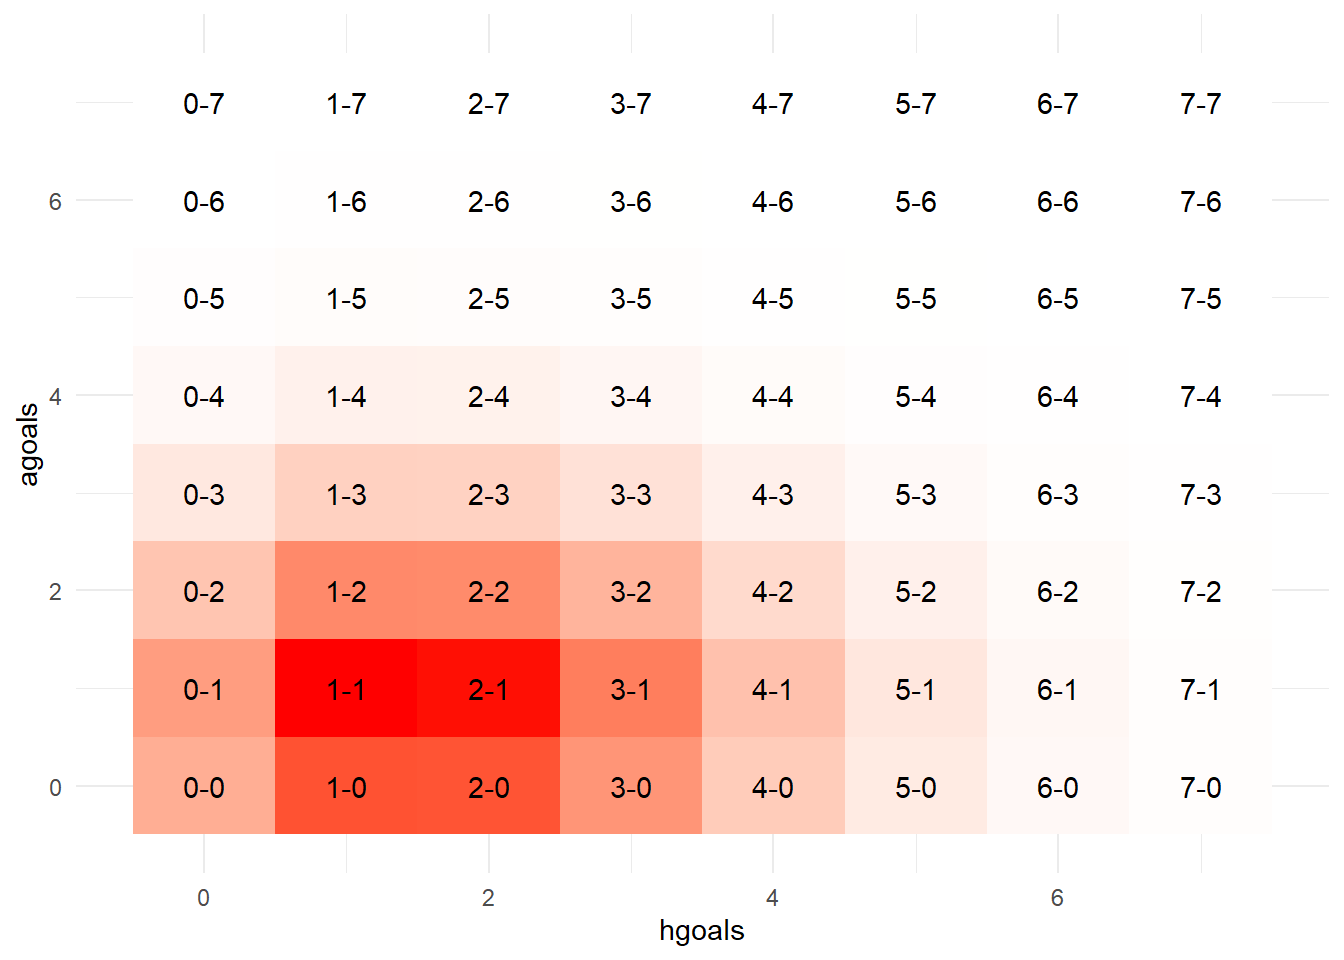
\includegraphics{2019-30-5-dixon-coles-2_files/figure-latex/example_tileplot-1.pdf}

Where we can see that the most common scorelines are low scoring
(football is a low scoring game), and slightly biased towards away goals
(i.e.~Arsenal are more likely to win than lose). The darkest (most
likely) tiles being 1-1 or a 2-1 Arsenal win seem very plausible given
our calculated λs earlier.

\begin{Shaded}
\begin{Highlighting}[]
\CommentTok{#want to predict over the whole fixture space}
\NormalTok{all_fixtures <-}\StringTok{ }\KeywordTok{bind_rows}\NormalTok{(fixtures, results)}
\end{Highlighting}
\end{Shaded}

\begin{verbatim}
## Warning in bind_rows_(x, .id): binding character and factor vector, coercing
## into character vector

## Warning in bind_rows_(x, .id): binding character and factor vector, coercing
## into character vector
\end{verbatim}

\begin{Shaded}
\begin{Highlighting}[]
\CommentTok{#get the lambda for each team per game}
\NormalTok{predictions <-}\StringTok{ }\KeywordTok{map2_df}\NormalTok{(all_fixtures}\OperatorTok{$}\NormalTok{home, all_fixtures}\OperatorTok{$}\NormalTok{away, }
\NormalTok{                       predict_results,}
\NormalTok{                       model)}
\end{Highlighting}
\end{Shaded}

\begin{verbatim}
## Warning in bind_rows_(x, .id): Unequal factor levels: coercing to character

## Warning in bind_rows_(x, .id): binding character and factor vector, coercing
## into character vector

## Warning in bind_rows_(x, .id): binding character and factor vector, coercing
## into character vector
\end{verbatim}

\begin{verbatim}
## Warning in bind_rows_(x, .id): Unequal factor levels: coercing to character
\end{verbatim}

\begin{verbatim}
## Warning in bind_rows_(x, .id): binding character and factor vector, coercing
## into character vector

## Warning in bind_rows_(x, .id): binding character and factor vector, coercing
## into character vector

## Warning in bind_rows_(x, .id): binding character and factor vector, coercing
## into character vector

## Warning in bind_rows_(x, .id): binding character and factor vector, coercing
## into character vector

## Warning in bind_rows_(x, .id): binding character and factor vector, coercing
## into character vector

## Warning in bind_rows_(x, .id): binding character and factor vector, coercing
## into character vector

## Warning in bind_rows_(x, .id): binding character and factor vector, coercing
## into character vector

## Warning in bind_rows_(x, .id): binding character and factor vector, coercing
## into character vector

## Warning in bind_rows_(x, .id): binding character and factor vector, coercing
## into character vector

## Warning in bind_rows_(x, .id): binding character and factor vector, coercing
## into character vector

## Warning in bind_rows_(x, .id): binding character and factor vector, coercing
## into character vector

## Warning in bind_rows_(x, .id): binding character and factor vector, coercing
## into character vector

## Warning in bind_rows_(x, .id): binding character and factor vector, coercing
## into character vector

## Warning in bind_rows_(x, .id): binding character and factor vector, coercing
## into character vector

## Warning in bind_rows_(x, .id): binding character and factor vector, coercing
## into character vector

## Warning in bind_rows_(x, .id): binding character and factor vector, coercing
## into character vector

## Warning in bind_rows_(x, .id): binding character and factor vector, coercing
## into character vector

## Warning in bind_rows_(x, .id): binding character and factor vector, coercing
## into character vector

## Warning in bind_rows_(x, .id): binding character and factor vector, coercing
## into character vector

## Warning in bind_rows_(x, .id): binding character and factor vector, coercing
## into character vector

## Warning in bind_rows_(x, .id): binding character and factor vector, coercing
## into character vector

## Warning in bind_rows_(x, .id): binding character and factor vector, coercing
## into character vector

## Warning in bind_rows_(x, .id): binding character and factor vector, coercing
## into character vector

## Warning in bind_rows_(x, .id): binding character and factor vector, coercing
## into character vector

## Warning in bind_rows_(x, .id): binding character and factor vector, coercing
## into character vector

## Warning in bind_rows_(x, .id): binding character and factor vector, coercing
## into character vector

## Warning in bind_rows_(x, .id): binding character and factor vector, coercing
## into character vector

## Warning in bind_rows_(x, .id): binding character and factor vector, coercing
## into character vector

## Warning in bind_rows_(x, .id): binding character and factor vector, coercing
## into character vector

## Warning in bind_rows_(x, .id): binding character and factor vector, coercing
## into character vector

## Warning in bind_rows_(x, .id): binding character and factor vector, coercing
## into character vector

## Warning in bind_rows_(x, .id): binding character and factor vector, coercing
## into character vector

## Warning in bind_rows_(x, .id): binding character and factor vector, coercing
## into character vector

## Warning in bind_rows_(x, .id): binding character and factor vector, coercing
## into character vector

## Warning in bind_rows_(x, .id): binding character and factor vector, coercing
## into character vector

## Warning in bind_rows_(x, .id): binding character and factor vector, coercing
## into character vector

## Warning in bind_rows_(x, .id): binding character and factor vector, coercing
## into character vector

## Warning in bind_rows_(x, .id): binding character and factor vector, coercing
## into character vector

## Warning in bind_rows_(x, .id): binding character and factor vector, coercing
## into character vector

## Warning in bind_rows_(x, .id): binding character and factor vector, coercing
## into character vector

## Warning in bind_rows_(x, .id): binding character and factor vector, coercing
## into character vector

## Warning in bind_rows_(x, .id): binding character and factor vector, coercing
## into character vector

## Warning in bind_rows_(x, .id): binding character and factor vector, coercing
## into character vector

## Warning in bind_rows_(x, .id): binding character and factor vector, coercing
## into character vector

## Warning in bind_rows_(x, .id): binding character and factor vector, coercing
## into character vector

## Warning in bind_rows_(x, .id): binding character and factor vector, coercing
## into character vector

## Warning in bind_rows_(x, .id): binding character and factor vector, coercing
## into character vector

## Warning in bind_rows_(x, .id): binding character and factor vector, coercing
## into character vector

## Warning in bind_rows_(x, .id): binding character and factor vector, coercing
## into character vector

## Warning in bind_rows_(x, .id): binding character and factor vector, coercing
## into character vector

## Warning in bind_rows_(x, .id): binding character and factor vector, coercing
## into character vector

## Warning in bind_rows_(x, .id): binding character and factor vector, coercing
## into character vector

## Warning in bind_rows_(x, .id): binding character and factor vector, coercing
## into character vector

## Warning in bind_rows_(x, .id): binding character and factor vector, coercing
## into character vector

## Warning in bind_rows_(x, .id): binding character and factor vector, coercing
## into character vector

## Warning in bind_rows_(x, .id): binding character and factor vector, coercing
## into character vector

## Warning in bind_rows_(x, .id): binding character and factor vector, coercing
## into character vector

## Warning in bind_rows_(x, .id): binding character and factor vector, coercing
## into character vector

## Warning in bind_rows_(x, .id): binding character and factor vector, coercing
## into character vector

## Warning in bind_rows_(x, .id): binding character and factor vector, coercing
## into character vector

## Warning in bind_rows_(x, .id): binding character and factor vector, coercing
## into character vector

## Warning in bind_rows_(x, .id): binding character and factor vector, coercing
## into character vector

## Warning in bind_rows_(x, .id): binding character and factor vector, coercing
## into character vector

## Warning in bind_rows_(x, .id): binding character and factor vector, coercing
## into character vector

## Warning in bind_rows_(x, .id): binding character and factor vector, coercing
## into character vector

## Warning in bind_rows_(x, .id): binding character and factor vector, coercing
## into character vector

## Warning in bind_rows_(x, .id): binding character and factor vector, coercing
## into character vector

## Warning in bind_rows_(x, .id): binding character and factor vector, coercing
## into character vector

## Warning in bind_rows_(x, .id): binding character and factor vector, coercing
## into character vector

## Warning in bind_rows_(x, .id): binding character and factor vector, coercing
## into character vector

## Warning in bind_rows_(x, .id): binding character and factor vector, coercing
## into character vector

## Warning in bind_rows_(x, .id): binding character and factor vector, coercing
## into character vector

## Warning in bind_rows_(x, .id): binding character and factor vector, coercing
## into character vector

## Warning in bind_rows_(x, .id): binding character and factor vector, coercing
## into character vector

## Warning in bind_rows_(x, .id): binding character and factor vector, coercing
## into character vector

## Warning in bind_rows_(x, .id): binding character and factor vector, coercing
## into character vector

## Warning in bind_rows_(x, .id): binding character and factor vector, coercing
## into character vector

## Warning in bind_rows_(x, .id): binding character and factor vector, coercing
## into character vector

## Warning in bind_rows_(x, .id): binding character and factor vector, coercing
## into character vector

## Warning in bind_rows_(x, .id): binding character and factor vector, coercing
## into character vector

## Warning in bind_rows_(x, .id): binding character and factor vector, coercing
## into character vector

## Warning in bind_rows_(x, .id): binding character and factor vector, coercing
## into character vector

## Warning in bind_rows_(x, .id): binding character and factor vector, coercing
## into character vector

## Warning in bind_rows_(x, .id): binding character and factor vector, coercing
## into character vector

## Warning in bind_rows_(x, .id): binding character and factor vector, coercing
## into character vector

## Warning in bind_rows_(x, .id): binding character and factor vector, coercing
## into character vector

## Warning in bind_rows_(x, .id): binding character and factor vector, coercing
## into character vector

## Warning in bind_rows_(x, .id): binding character and factor vector, coercing
## into character vector

## Warning in bind_rows_(x, .id): binding character and factor vector, coercing
## into character vector

## Warning in bind_rows_(x, .id): binding character and factor vector, coercing
## into character vector

## Warning in bind_rows_(x, .id): binding character and factor vector, coercing
## into character vector

## Warning in bind_rows_(x, .id): binding character and factor vector, coercing
## into character vector

## Warning in bind_rows_(x, .id): binding character and factor vector, coercing
## into character vector

## Warning in bind_rows_(x, .id): binding character and factor vector, coercing
## into character vector

## Warning in bind_rows_(x, .id): binding character and factor vector, coercing
## into character vector

## Warning in bind_rows_(x, .id): binding character and factor vector, coercing
## into character vector

## Warning in bind_rows_(x, .id): binding character and factor vector, coercing
## into character vector

## Warning in bind_rows_(x, .id): binding character and factor vector, coercing
## into character vector

## Warning in bind_rows_(x, .id): binding character and factor vector, coercing
## into character vector

## Warning in bind_rows_(x, .id): binding character and factor vector, coercing
## into character vector

## Warning in bind_rows_(x, .id): binding character and factor vector, coercing
## into character vector

## Warning in bind_rows_(x, .id): binding character and factor vector, coercing
## into character vector

## Warning in bind_rows_(x, .id): binding character and factor vector, coercing
## into character vector

## Warning in bind_rows_(x, .id): binding character and factor vector, coercing
## into character vector

## Warning in bind_rows_(x, .id): binding character and factor vector, coercing
## into character vector

## Warning in bind_rows_(x, .id): binding character and factor vector, coercing
## into character vector
\end{verbatim}

\begin{Shaded}
\begin{Highlighting}[]
\CommentTok{#calc out probabilities and bind up}
\NormalTok{all_predictions <-}\StringTok{ }\KeywordTok{map2_df}\NormalTok{(predictions}\OperatorTok{$}\NormalTok{e_hgoal, predictions}\OperatorTok{$}\NormalTok{e_agoal, }\ControlFlowTok{function}\NormalTok{(lambda_home, lambda_away, max_goals) \{}
\NormalTok{  hgoal_prob <-}\StringTok{ }\KeywordTok{dpois}\NormalTok{(}\DecValTok{0}\OperatorTok{:}\NormalTok{max_goals, lambda_home) }\OperatorTok\StringTok{ `}\DataTypeTok{names<-}\StringTok{`}\NormalTok{(}\DecValTok{0}\OperatorTok{:}\NormalTok{max_goals)}
\NormalTok{  agoal_prob <-}\StringTok{ }\KeywordTok{dpois}\NormalTok{(}\DecValTok{0}\OperatorTok{:}\NormalTok{max_goals, lambda_away) }\OperatorTok\StringTok{ `}\DataTypeTok{names<-}\StringTok{`}\NormalTok{(}\DecValTok{0}\OperatorTok{:}\NormalTok{max_goals)}
  \KeywordTok{outer}\NormalTok{(hgoal_prob, agoal_prob) }\OperatorTok
\StringTok{      }\KeywordTok{as.data.frame}\NormalTok{() }\OperatorTok\StringTok{ }
\StringTok{      }\KeywordTok{gather}\NormalTok{() }\OperatorTok\StringTok{ }
\StringTok{      }\KeywordTok{rownames_to_column}\NormalTok{(}\StringTok{"row"}\NormalTok{) }\OperatorTok
\StringTok{      }\KeywordTok{mutate}\NormalTok{(}\DataTypeTok{hgoal =} \KeywordTok{as.numeric}\NormalTok{(row) }\OperatorTok\StringTok{ }\NormalTok{(max_goals}\OperatorTok{+}\DecValTok{1}\NormalTok{)}\OperatorTok{-}\DecValTok{1}\NormalTok{) }\OperatorTok\StringTok{ }
\StringTok{      }\KeywordTok{mutate}\NormalTok{(}\DataTypeTok{hgoal =} \KeywordTok{case_when}\NormalTok{(hgoal }\OperatorTok{<}\StringTok{ }\DecValTok{0} \OperatorTok{~}\StringTok{ }\NormalTok{max_goals, }\OtherTok{TRUE} \OperatorTok{~}\StringTok{ }\NormalTok{hgoal),}
             \DataTypeTok{agoal =} \KeywordTok{as.numeric}\NormalTok{(key)) }\OperatorTok
\StringTok{      }\KeywordTok{select}\NormalTok{(}\DataTypeTok{hgoal_name =}\NormalTok{ hgoal, }\DataTypeTok{agoal_name =}\NormalTok{ agoal, }\DataTypeTok{prob =}\NormalTok{ value)}
\NormalTok{\}, max_goals) }\OperatorTok
\StringTok{  }\KeywordTok{cbind}\NormalTok{(all_fixtures[}\KeywordTok{rep}\NormalTok{(}\KeywordTok{seq_len}\NormalTok{(}\KeywordTok{nrow}\NormalTok{(all_fixtures)), }\DataTypeTok{each=}\NormalTok{(max_goals}\OperatorTok{+}\DecValTok{1}\NormalTok{)}\OperatorTok{^}\DecValTok{2}\NormalTok{),], .)}

\CommentTok{#plot again}
\NormalTok{p3 <-}\StringTok{ }\NormalTok{all_predictions }\OperatorTok
\StringTok{  }\CommentTok{#filter only a few out to scale plot }
\StringTok{  }\KeywordTok{filter}\NormalTok{(home }\OperatorTok\StringTok{ }\KeywordTok{c}\NormalTok{(}\StringTok{"Arsenal"}\NormalTok{, }\StringTok{"Coventry_City"}\NormalTok{, }\StringTok{"Enfield_Town"}\NormalTok{),}
\NormalTok{         away }\OperatorTok\StringTok{ }\KeywordTok{c}\NormalTok{(}\StringTok{"Arsenal"}\NormalTok{, }\StringTok{"Coventry_City"}\NormalTok{, }\StringTok{"Enfield_Town"}\NormalTok{)) }\OperatorTok
\StringTok{  }\KeywordTok{ggplot}\NormalTok{(}\KeywordTok{aes}\NormalTok{(}\DataTypeTok{x =}\NormalTok{ hgoal_name, }\DataTypeTok{y =}\NormalTok{ agoal_name, }\DataTypeTok{fill =}\NormalTok{ prob)) }\OperatorTok{+}
\StringTok{  }\KeywordTok{geom_tile}\NormalTok{() }\OperatorTok{+}
\StringTok{  }\KeywordTok{geom_point}\NormalTok{(}\KeywordTok{aes}\NormalTok{(}\DataTypeTok{x =}\NormalTok{ hgoal, }\DataTypeTok{y =}\NormalTok{ agoal), }
             \DataTypeTok{colour =} \StringTok{"blue"}\NormalTok{, }\DataTypeTok{size =} \DecValTok{10}\NormalTok{, }\DataTypeTok{alpha =} \FloatTok{0.5} \OperatorTok{/}\StringTok{ }\NormalTok{max_goals}\OperatorTok{^}\DecValTok{2}\NormalTok{) }\OperatorTok{+}
\StringTok{  }\KeywordTok{geom_text}\NormalTok{(}\KeywordTok{aes}\NormalTok{(}\DataTypeTok{label =} \KeywordTok{paste}\NormalTok{(hgoal_name, agoal_name, }\DataTypeTok{sep =} \StringTok{"-"}\NormalTok{))) }\OperatorTok{+}
\StringTok{  }\KeywordTok{scale_fill_gradient2}\NormalTok{(}\DataTypeTok{low =} \StringTok{"white"}\NormalTok{, }\DataTypeTok{high =} \StringTok{"red"}\NormalTok{, }\DataTypeTok{guide =} \OtherTok{FALSE}\NormalTok{) }\OperatorTok{+}
\StringTok{  }\KeywordTok{labs}\NormalTok{(}
    \DataTypeTok{title =} \StringTok{"predictions for final score across all fixtures"}\NormalTok{,}
    \DataTypeTok{y =} \StringTok{"away goals"}\NormalTok{,}
    \DataTypeTok{x =} \StringTok{"home goals"}\NormalTok{) }\OperatorTok{+}
\StringTok{  }\KeywordTok{theme_minimal}\NormalTok{() }\OperatorTok{+}
\StringTok{  }\KeywordTok{facet_grid}\NormalTok{(away}\OperatorTok{~}\NormalTok{home)}

\NormalTok{p3}
\end{Highlighting}
\end{Shaded}

\begin{verbatim}
## Warning: Removed 384 rows containing missing values (geom_point).
\end{verbatim}

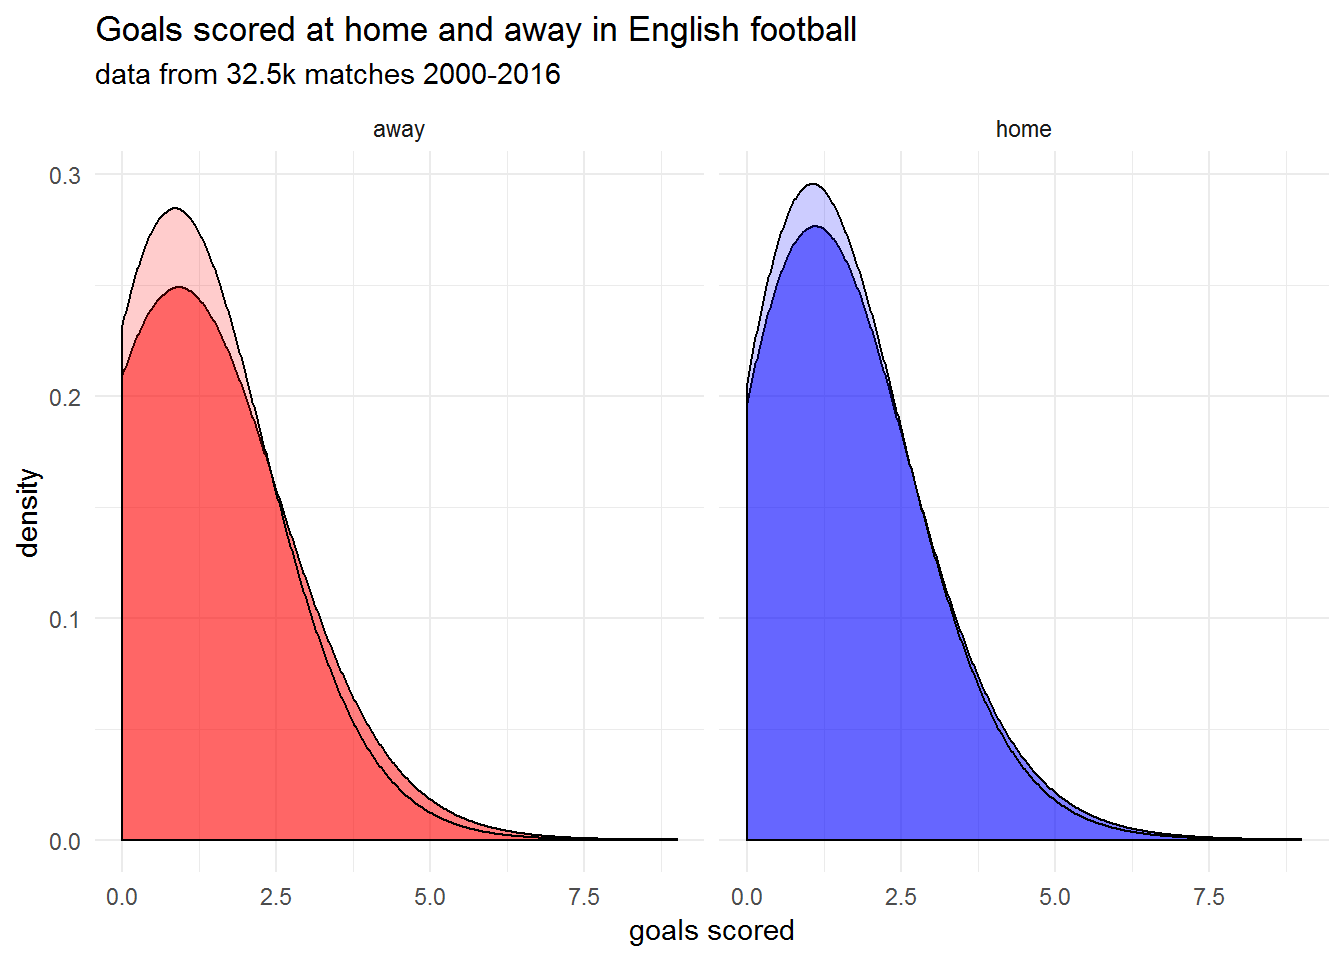
\includegraphics{2019-30-5-dixon-coles-2_files/figure-latex/unnamed-chunk-3-1.pdf}

\hypertarget{so-what}{%
\subsection{So what?}\label{so-what}}

These graphs are nice, but whats important is what they show: \emph{we
have a way to quantify how likely any result is in a match between two
given teams}. Why is this useful

\begin{itemize}
\tightlist
\item
  Firstly, we can use the output of this to build betting models. Given
  the odds on final scores for any match, we can hedge effectively by
  betting on (e.g.) the five overwhelmingly most likely results.
\item
  Secondly, we can simulate leagues. This is
  \href{https://www.bloomberg.com/graphics/2020-coronavirus-european-football/}{perhaps
  especially of interest given the context of writing this post}. I'm
  going to focus on this application because I don't bet on football,
  and also because it's hard to get a nice database of odds at the
  moment given the aforemention situation.
\end{itemize}

\href{https://www.youtube.com/watch?v=DYb8gS-wDrM}{The Verve - Monte
Carlo}

We can do this using a technique called
\href{https://en.wikipedia.org/wiki/Monte_Carlo_method}{Monte Carlo
simulation}. There are lots of good explanation of the technique on the
internet, but it basically boils down to this:

\_if events follow a known distribution*, you can sample these events
lots of times to get stochastic guesstimates, but over many samples you
will reproduce exactly that distribution\_

*a Poisson distribution for the expected number of goals scored in our
case

For football, this means that while on an individual match level results
are noisy (sometimes better teams lose!), if we simulate matches lots
and lots of times, eventually they should converge to the `truth'*

*as defined by our Poisson distribution (which may or may not be a
good/accurate `truth' but go with it for now).

\end{document}
